\section{Related Work}

\subsection{Video diffusion}
% \textbf{3D-aware generation}

% https://zqh0253.github.io/wvd/
% MotionShop: Zero-Shot Motion Transfer in Video Diffusion Models with Mixture of Score Guidance
% Generative rendering
In recent years, the success of diffusion models in image generation~\cite{ho2020denoising, rombach2022high, peebles2023scalable} has sparked interest in exploring video generation~\cite{ho2022video, he2022latent, blattmann2023stable, chen2023videocrafter1, chen2024videocrafter2, brooks2024video, yang2024cogvideox, keling, kong2024hunyuanvideo, lin2024open, opensora, xing2025dynamicrafter,guo2023animatediff}. VDM~\cite{ho2022video} is the first work to explore the feasibility of diffusion in the field of video generation. SVD~\cite{blattmann2023stable} introduces a unified strategy for training a robust video generation model. Sora~\cite{brooks2024video}, through training on extensive video data, suggests that scaling video generation models is a promising path towards building general-purpose simulators of the physical world. CogVideo-X~\cite{yang2024cogvideox}, 
VideoCrafter~\cite{chen2023videocrafter1,chen2024videocrafter2}, DynamiCrafter~\cite{xing2025dynamicrafter},  Keling~\cite{keling}, and Hunyuan~\cite{kong2024hunyuanvideo} have demonstrated impressive video generation performance with strong temporal consistency. 


\textbf{Controllable video generation}. Existing works still lack an effective way to control the generation process. 
There are many works~\cite{wang2024motionctrl,he2024cameractrl,polyak2024movie,he2024id,yuan2024identity,wang2024boximator,huang2023fine,guo2024sparsectrl,namekata2024sg,ma2024trailblazer,ma2024follow,yu2024viewcrafter,ma2024follow,qiu2024freetraj} that introduce a specific control signal in the video generation process which can only achieve one control type like identity preserving, camera control, and motion transfer. 
Our method is more versatile in various video control types by using a 3D-aware video generation with 3D tracking videos as conditions.


% \subsection{Control signals}
% There are numerous works that introduce specific control signals into the video generation process. \cite{wang2024motionctrl,he2024cameractrl} incorporate specific camera trajectories to control video content. \cite{polyak2024movie,he2024id,yuan2024identity} use human images as prompts to maintain specified human identities. \cite{wang2024boximator,huang2023fine,guo2024sparsectrl,namekata2024sg,ma2024trailblazer,ma2024follow} manage the direction of object movement by integrating motion signals. In this paper, we propose using 3D tracking, as introduced in ~\cite{xiao2024spatialtracker}, as a control signal. With the help of 3D tracking, our method can achieve more fine-grained control and effectively maintain both temporal and spatial consistency.


\subsection{Controlled video generation}
% We review the following five types of controlled video generation tasks with a 3D tracking video as a generation condition: animating meshes to videos, camera control, motion retargeting, physics-aware video generation, and object manipulation. 
We review the following 4 types of controlled video generation.

\textbf{Animating meshes to videos.}
Animating meshes to videos aims to texture meshes. Several works~\cite{cao2023texfusion,richardson2023texture,wang2023breathing,cai2024generative} have demonstrated the feasibility of mesh texturization using powerful diffusion models.
TexFusion~\cite{cao2023texfusion} applies the diffusion model’s denoiser on a set of 2D renders of the 3D object, optimizing an intermediate neural color field to output final RGB textures. 
TEXTure~\cite{richardson2023texture} introduces a dynamic trimap representation and a novel diffusion sampling process, leveraging this trimap to generate seamless textures from various views. 
G-Rendering~\cite{cai2024generative} takes a dynamic mesh as input. To preserve consistency, G-Rendering employs UV-guided noise initialization and correspondence-aware blending of both pre- and post-attention features. Following G-Rendering, our method also targets dynamic meshes, utilizing a diffusion model as a shader to incorporate realistic texture information. Unlike G-Rendering, which preserves consistency at the noise and attention levels, our approach leverages 3D tracking videos as supplementary information, integrating them into the diffusion model to ensure both temporal and spatial consistency.

\textbf{Camera control.}
Camera control~\cite{wang2024motionctrl,he2024cameractrl,zheng2024cami2v,yu2024viewcrafter,bahmani2024ac3d,yang2024direct,xiao2024trajectory,geng2024motion,wang2024cpa} is an important capability for enhancing the realism of generated videos and increasing user engagement by allowing customized viewpoints. Recently, many efforts have been made to introduce camera control in video generation. MotionCtrl~\cite{wang2024motionctrl} incorporates a flexible motion controller for video generation, which can independently or jointly control camera motion and object motion in generated videos. CameraCtrl~\cite{he2024cameractrl} adopts Plücker embeddings~\cite{sitzmann2021light} as the primary form of camera parameters, enabling the ViewCrafter~\cite{yu2024viewcrafter} employs a point-based representation for free-view rendering, enabling precise camera control. AC3D~\cite{bahmani2024ac3d} optimizes pose conditioning schedules during training and testing to accelerate convergence and restricts the injection of camera conditioning to specific positions, reducing interference with other meaningful video features. %TrajAttn~\cite{xiao2024trajectory} introduces an auxiliary branch, termed trajectory attention, to ensure both precise camera control and new content generation capabilities. 
CPA~\cite{wang2024cpa} incorporates a Sparse Motion Encoding Module to embed the camera pose information and integrating the embedded motion information via temporal attention.
Our method aims to use 3D tracking videos as an intermediary to achieve precise and consistent camera control.
% https://snap-research.github.io/ac3d/?s=09
% https://xizaoqu.github.io/trajattn/
%yu2024viewcrafter

\textbf{Motion transfer.}
Motion transfer~\cite{esser2023structure,geyer2023tokenflow,pondaven2024video,wang2024motionctrl,wang2024videocomposer,park2024spectral,yatim2024space,meral2024motionflow,geng2024motion} aims to synthesize novel videos by following the motion of the original one. Gen-1~\cite{esser2023structure} employs depth estimation results~\cite{ranftl2020towards, bochkovskii2024depth, lu2024align3r} to guide the motion. TokenFlow~\cite{geyer2023tokenflow} achieves consistent motion transfer by enforcing consistency in the diffusion feature space. MotionCtrl~\cite{wang2024motionctrl} also achieves motion transfer by incorporating a motion controller. DiTFlow~\cite{pondaven2024video} proposes Attention Motion Flow as guidance for motion transfer on DiTs~\cite{peebles2023scalable}. Motion Prompting~\cite{geng2024motion} utilizes 2D motions as prompts to realize impressive motion transfer. Unlike these approaches, our method employs 3D tracking as guidance for motion transfer, enabling a more comprehensive capture of each object's motion and the relationships between them within the video. This ensures accurate and globally consistent geometric and temporal consistency.
% https://ditflow.github.io/
% https://motion-prompting.github.io/

\begin{figure*}
    \centering
    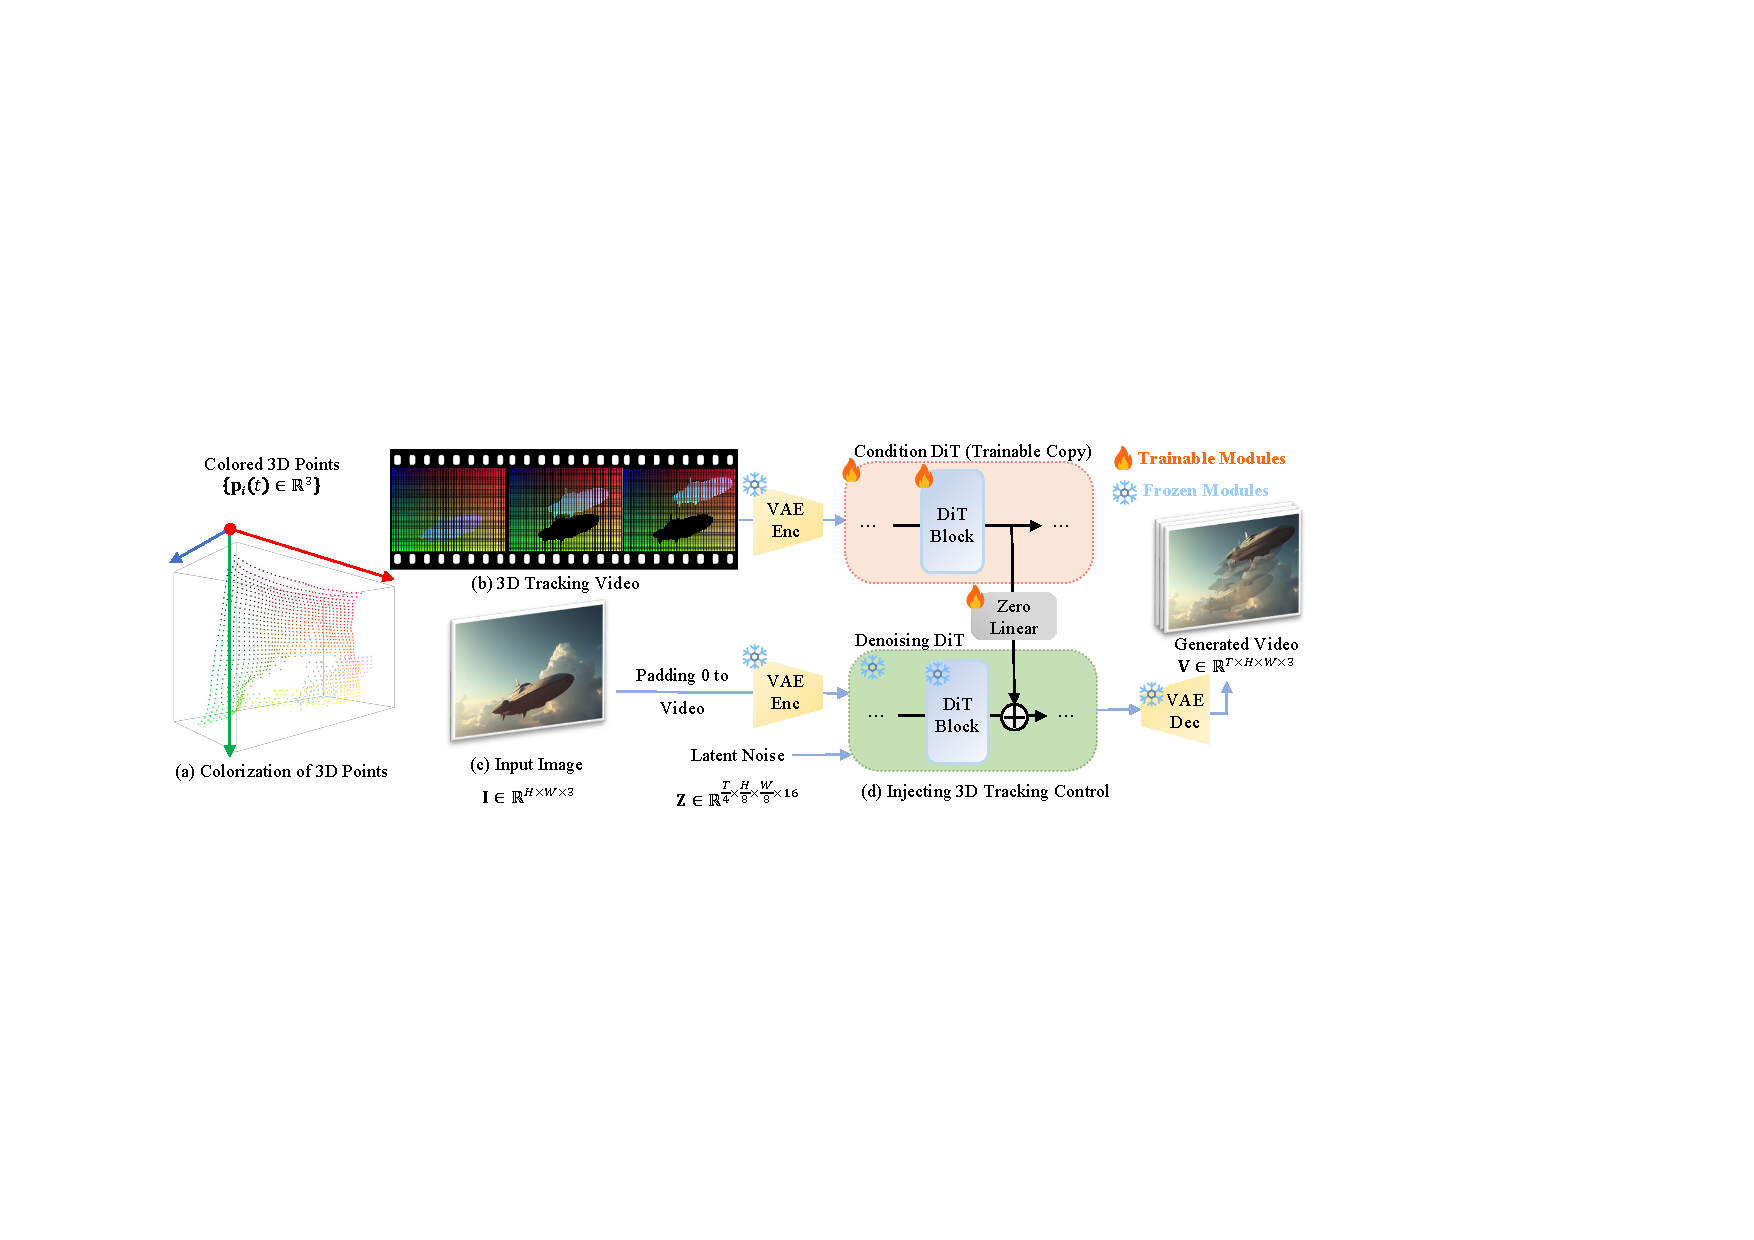
\includegraphics[width=\textwidth]{pictures/pipeline.pdf}
    \caption{\textbf{Architecture of \methodname}. (a) We colorize dynamic 3D points according to their coordinates to get (b) a 3D tracking video. (c) The input image and the 3D tracking video are processed by (d) a transformer-based latent diffusion with a variational autoencoder (VAE). The 3D tracking video is processed by a trainable copy of the denoising DiT and zero linear layers are used to inject the condition features from 3D tracking videos into the denoising process.}
    \label{fig:pipe}
\end{figure*}

% \textbf{Physics-aware video generation.}
% Physics-aware video generation~\cite{xie2024physgaussian,zhang2025physdreamer,liu2025physgen, tan2024physmotion} aims to create outputs that conform to fundamental physical principles.   
% %Previous studies~\cite{xie2024physgaussian,jiang2024vr,liu2025physgen,zhang2025physdreamer,tan2024physmotion} have used physics simulators to model physical dynamics and render videos via differentiable rendering or Gaussian Splatting. PhysGaussian~\cite{xie2024physgaussian} and VR-GS~\cite{jiang2024vr} leverage simulators such as MPM~\cite{jiang2016material}, XPBD~\cite{macklin2016xpbd} to achieve physics-driven video generation. 
% PhysGaussian~\cite{xie2024physgaussian} utilizes simulators like MPM~\cite{jiang2016material} to achieve realistic, physics-driven video synthesis.
% PhysDreamer~\cite{zhang2025physdreamer} leverages Score Distillation Sampling (SDS)~\cite{poole2022dreamfusion} to distill video diffusion knowledge, enabling static 3D objects to exhibit interactive dynamics.
% PhysGen~\cite{liu2025physgen} captures the geometry, materials, and physical parameters of images, and employs rigid-body physics alongside inferred parameters to simulate realistic behaviors.
% PhysMotion~\cite{tan2024physmotion} reconstructs a 3D Gaussian representation from a single image, leveraging it to create physics-driven videos.
% Using 3D tracking as an intermediate medium, our method leverages Blender’s physics simulation to generate physically correct meshes, which are subsequently converted into 3D tracking videos to guide \methodname for physics-aware video generation.

\textbf{Object manipulation.} 
Object manipulation refers to versatile object movement control for image-to-video generation. Different from camera control, which focuses on changes in perspective, object manipulation emphasizes the movement of the objects themselves. 
Currently, mainstream methods~\cite{chen2023motion,li2024image,mou2024revideo,teng2023drag,wang2024motionctrl,yin2023dragnuwa,jain2024peekaboo,ma2024trailblazer,qiu2024freetraj,wang2024boximator,yang2024direct,geng2024motion} typically achieve object manipulation by utilizing directed trajectories or modeling the relationships between bounding boxes with specific semantic meanings. However, these methods primarily rely on 2D guidance to represent the spatial movement of target objects, which often fails to accurately capture user intent and frequently results in distorted outputs. ObjCtrl-2.5D~\cite{wang2024objctrl} tries to address this limitation by extending 2D trajectories with depth information, creating a single 3D trajectory as the control signal. Better than the single 3D trajectory, our method leverages 3D tracking videos, which offer greater details and more effectively represent the motion relationships between foreground and background for more precise and realistic object manipulation.

% ObjCtrl-2.5D: Training-free Object Control with Camera Poses


\textbf{Concurrent works}. %\cite{jeong2024track4gen, pandey2024motion, geng2024motion} are concurrent works also aiming to achieve spatiotemporal content control.
Recently, several works~\cite{geng2024motion, niu2025mofa, koroglu2024onlyflow, jeong2024track4gen, shi2024motion, lei2024animateanything,feng2024i2vcontrol,zhang2024world} have explored utilizing motion as control signals. These approaches can be broadly categorized into two groups: 2D motion-based and 3D motion-based methods.  
\cite{koroglu2024onlyflow, shi2024motion,lei2024animateanything} leverage 2D optical flow to condition motion, while \cite{niu2025mofa,geng2024motion,jeong2024track4gen} utilize 2D tracks, which are sparser than optical flow, to track or control video motion. 
\cite{zhang2024world} learns to generate 3D coordinates in the video diffusion model, which 3D awareness. \cite{feng2024i2vcontrol} lifts videos into 3D space and extracts the motion of 3D points, enabling a more accurate capture of spatial relationships between objects and supporting tasks such as object manipulation and camera control. Our method, \methodname, also leverages recent tracking methods~\cite{xiao2024spatialtracker,zhang2024protracker} to construct videos. However, we extend the applicability by unifying a broader range of control tasks, including mesh-to-video generation and motion transfer.
% Furthermore, we showcase the ability to transfer an animated 3D mesh into a video.
% \cite{jeong2024track4gen} employs explicit supervision in terms of spatial tracking at the feature level. \cite{pandey2024motion} uses a flow generator guided by energy functions to discover various motions and then uses these motions to control the generation process. \cite{geng2024motion} utilizes 2D motions as prompts for video generation and also shows its applications in various control tasks. In contrast to all these works that are 2D motion-based, our method \methodname is inspired by CG pipelines to represent the video motion in the 3D space and we demonstrate the results of transferring an animated 3D mesh into a video. 
% DAS incorporates a 3D tracking video into the diffusion model while other methods mainly employ explicit or implicit supervision at the 2D level.
